\begin{figure}
\centering
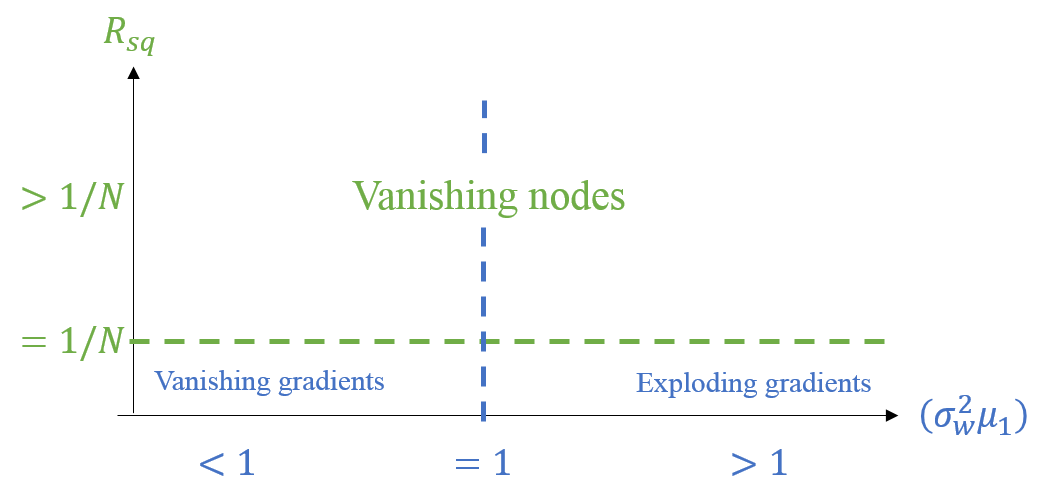
\includegraphics[width=0.9\textwidth]{theo}
\caption[The schematic diagram for deep neural network architectures]
{The schematic diagram for deep neural network architectures.
To avoid the deep network gradients from exploding or vanishing, it is suggested that the condition 
$(\sigma_w^2\mu_1)=1$ should be met.
For vanishing nodes problem, the VNI $R_{sq}$ of the network shall not increases to 1 as the network
depth $L$ goes deeper, otherwise the representation power of the network will be insufficient for 
the training task.
That is, to overcome the two obstacles of training a very deep network,
the best network setting is located at the intersection of vertical and horizontal dashed line.}
\label{fig:sec6_theo1}
\setlength{\belowcaptionskip}{-10pt}
\end{figure}